%---------- Inleiding ---------------------------------------------------------

\section{Introductie}%
\label{sec:introductie}
In de afgelopen jaren zijn er heel wat nieuwe javascript runtime-omgevingen geïntroduceerd. 
Echter worden weinig van deze nieuwe environments effectief gebruikt. 
Zo toont onderzoek van ~\textcite{Greif2022} aan dat 93.6\% van de 29888 bevraagden Node.js regulier gebruiken.
Dit tegenover de 11.2\% en 4.3\% van de mensen die respectievelijk Deno en Bun geregeld gebruiken.
Momenteel wordt Node.JS nog altijd als standaard gebruikt bij elk project. 
Er zijn echter nog tal van andere javascript runtime-omgevingen, zoals bovengenoemde Bun en Deno, 
die in staat zijn om specifieke noden te vervullen waar Node.js niet kan aan voldoen.
Het doel van deze studie is te onderzoeken of één van deze nieuwe frameworks een correcte plaatsvervanger is voor Node.js 
binnen de ontwikkeling van performante web applicaties bij Codifly. Hierbij spelen verschillende aspecten een rol.
Is het nieuwe framework performanter? Wat is het verschil tussen de package managers?
Hoe complex is het nieuwe framework tegenover Node.js?
Om deze vragen te beantwoorden wordt de 
performantie en complexiteit tussen Node.js en het nieuwe framework Bun vergeleken aan de hand van een proof-of-concept.
Hierbij wordt de performantie zowel gemeten bij simpele applicaties zoals het uitvoeren van logische berekeningen
als meer complexe applicaties waarbij netwerk verzoeken worden gebruikt.
In wat volgt wordt eerst een overzicht gegeven van de actuele ontwikkelingen binnen het
onderzoeksdomein aan de hand van een literatuurstudie, waarna de methodologie wordt besproken.
Ten laatste worden de resultaten van de vergelijking alsook de conclusie besproken.


%---------- Stand van zaken ---------------------------------------------------

\section{State-of-the-art}%
\label{sec:state-of-the-art}
% Voor literatuurverwijzingen zijn er twee belangrijke commando's:
% \autocite{KEY} => (Auteur, jaartal) Gebruik dit als de naam van de auteur
%   geen onderdeel is van de zin.
% \textcite{KEY} => Auteur (jaartal)  Gebruik dit als de auteursnaam wel een
%   functie heeft in de zin (bv. ``Uit onderzoek door Doll & Hill (1954) bleek
%   ...'')
Javascript vormt de basis voor alle Javascript runtime-omgevingen. 
Het is een geïnterpreteerde programmeertaal dat vooral bekend is bij front-end web development voor web pagina's ~\autocite{Mozilla2023}.
Echter kan het ook buiten browser omgevingen gebruikt worden met behulp van javascript runtime-omgevingen zoals Node.js,Bun en Deno ~\autocite{Mozilla2023}.
Zo een omgeving bestaat uit alle componenten om javascript correct te laten werken ~\autocite{Christopher}. 
Het bevat een JavaScript engine, WEB API's en een callback queue ~\autocite{Christopher}. 
Deze runtime zal dan javascript code omzetten in code die verstaanbaar is voor de computer.
De omgeving specificeert waar dit wordt gedaan, dit kan in een browser maar ook in andere omgevingen.
De afgelopen jaren is het aantal van deze soort omgevingen sterk toegenomen. 
De meest bekende en oudste is Node.js. 
Node.js is een server-side framework dat wordt gebruikt voor schaalbare applicaties te maken ~\autocite{Gackenheimer2013}.
In het boek van ~\textcite{Ali2013} wordt verteld hoe Node.js zich onderscheidt van andere platformen door het gebruik van een event loop. 
Wanneer in Node.js een I/O operatie wordt verwerkt zal een gebeurtenis worden uitgezonden. 
De event loop zal continu kijken of er zo gebeurtenissen voorkomen, 
en wanneer dit zo is zal het deze plaatsen in de event wachtrij. 
De event loop zal dan deze wachtrij doorgaan en één per één de event handlers uitvoeren. 
Dit laat toe om I/O operaties asynchroon te maken.
De JavaScript code binnenin Node.js wordt uitgevoerd door de V8 JavaScript engine, 
dezelfde engine die toelaat om JavaScript uit te voeren in Chrome ~\autocite{Syed2014}.
Hierbij wordt gebruikgemaakt van een call stack en een heap. 
De call stack is de plaats waar de code wordt uitgevoerd,terwijl de heap de plaats is waar alle nodige objecten worden opgeslagen ~\autocite{Christopher}.
Doordat JavaScript files steeds groter werden, werd in 2009 CommonJS geïntroduceerd. 
Dit specificeert een simpele API om modules te declareren die werken buiten de browser ~\autocite{Osmani2012}.
Hierbij is een module een stuk herbruikbare code dat kan gebruikt worden in  andere code ~\autocite{Osmani2012}.
Node.js volgt de CommonJS module specificatie, waarbij elk bestand zijn eigen module vormt ~\autocite{Syed2014}.
Buiten zelf modules te schrijven, bestaan er ook modules die geschreven zijn door andere mensen. 
Deze zijn te vinden in de Node Package Manager (NPM) ~\autocite{Wittern2016}. 
Deze modules kunnen dan gebruikt worden door andere mensen in hun eigen project ~\autocite{Ali2013}.

Performantie is één van de belangrijkste zaken bij een server-side framework. Daarom is Node.js dankzij zijn 
event-gedreven I/O model een veelvoorkomende keuze als het gaat om server-side frameworks. 
Echter wil Bun dit veranderen door nog meer focus te leggen op snelheid en performantie. 
Om dit te bereiken maakt Bun gebruik van JavaScriptCore in plaats van de V8 JavaScript engine ~\autocite{McDonnel2023}.
Dit is de ingebouwde engine voor WebKit, een web browser engine die wordt gebruikt op macOS en IOS ~\autocite{Pizlo2020}.
Door het gebruik van de JavaScriptCore engine zou Bun 4 keer sneller kunnen opstarten dan Node.js ~\autocite{McDonnel2023}.
Bun bevat daarnaast ook een test runner,script runner en een Node.js compatibele package manager, die volgens ~\textcite{McDonnel2023} 
allemaal significant sneller zijn dan bestaande applicaties zoals Node.js en Deno.
Een ander verschil tussen Node.js en Bun is de ingebouwde support voor TypeScript en JSX. 
Terwijl bij Node.js je hiervoor aparte packages nodig hebt, 
zal bij Bun de transpiler deze bestanden automatisch converteren naar vanilla Javascript.

Doordat Bun redelijk nieuw is, zijn er nog maar weinig onderzoeken over gedaan.
Eén van deze onderzoeken werd uitgevoerd door ~\textcite{Feroj2023}.
Hierbij werd de performantie tussen Node.js en Bun vergeleken op basis van verschillende performantie attributen. 
Deze omvatten geheugengebruik, antwoordtijd en de algemene uitvoeringstijd. 
Voor het testen van netwerk verzoeken werd bij beiden gebruikgemaakt van Bombardier. Hierbij werden in 3 aparte scenario's, 
10 miljoen verzoeken gemaakt met eerst 10 gelijktijdige connecties, dan 100 gelijktijdige connecties en
uiteindelijk 500 gelijktijdige connecties. Hierbij kon de onderzoeker de performantie van de servers evalueren 
aan de hand van responstijd en doorvoer. Aanvullend werden ook de geheugengebruik pieken bepaald.
Daarnaast werd ook getest hoe beide runtimes een alleenstaand script afhandelen. 
Dit werd gedaan aan de hand van Hyperfine, een command-line process benchmark hulpmiddel. 
Hierbij werd de executie tijd gemeten in zowel Bun als Node.js voor het berekenen van Fibonacci nummers.
Het eerste resultaat toont het verschil in geheugengebruik tussen Bun en Node.js. 
Hierbij heeft Bun consistent een lager geheugengebruik tegenover Node.js en toont het aan dat Bun een beter geheugenbeheer heeft.
De onderzoeker merkt op dat de oorzaak hiervan ligt bij Bun's gebruik van Zig, 
een programmeertaal gekend voor zijn effectiviteit en geheugenbeheer. 
Ook op vlak van executie tijd, responstijd en doorvoer presteerde Bun consistent beter dan Node.js. 
Deze resultaten tonen aan dat Bun algemeen beter presteert in zowel het afhandelen van netwerk verzoeken 
als het uitvoeren van computationele taken.
De onderzoeker merkt echter ook op dat de keuze van een runtime niet alleen kan bepaald worden op basis van performantie. 
Andere factoren, die hier niet getest zijn, zoals beveiling, stabiliteit en onderhoudbaarheid dragen ook bij tot de keuze. 
Ook waren de geteste programma's redelijk simpel waardoor de resultaten mogelijks niet accuraat zijn voor complexere omgevingen.
Verder onderzoek zou ook baat hebben om rekening te houden met verschillende omstandigheden, 
zoals CPU-gebonden en I/O-gebonden processen.

Een ander nieuw framework is Deno. 
Dit framework werd geïntroduceerd door ~\textcite{Dahl2021}, de maker van Node.js.
Met Deno wil hij nieuw leven inblazen in het ecosysteem door middel van een modern, productief programmeer systeem aan te bieden dat zich houdt aan browser API's.
Net zoals Node.js gebruikt Deno de V8 Javascript engine ~\autocite{DenoLand2023}. Echter werd Deno ontwikkeld in Rust, terwijl Node in C en C++ ~\autocite{DenoLand2023}. 
Eén van de kenmerken van Deno is de beveiliging. Zo is er standaard runtime-beveiliging, 
waarbij je als ontwikkelaar expliciet moet toestaan dat code toegang mag krijgen tot gevoelige API's ~\autocite{DenoLand2023}.
Technisch gezien heeft Deno geen package manager. Het maakt gebruik van URL's om externe modules te importeren ~\autocite{DenoLand2023}.
Het voordeel hierbij is dat wanneer je een module importeert, deze automatisch wordt gecached ~\autocite{DenoLand2023}.

Doordat Deno redelijk recent, zijn er ook hier nog maar weinig onderzoeken over gedaan.
Eén van deze onderzoeken werd uitgevoerd door ~\textcite{VanKerkvoorde2021}. 
Hierbij werd Node.js vergeleken met Deno op verschillende vlakken zoals performantie en beveiliging.
Op vlak van beveiliging scoort Deno beter dan Node.js door middel van standaard geen toegang te geven tot de folderstructuur en omgeving. 
Ook kunnen er standaard geen netwerk connecties worden gemaakt. 
Voor de performantie te testen van beide frameworks werd allereerst een logica test uitgevoerd op beiden. 
De onderzoeker heeft hierbij ondervonden dat Deno gemiddeld 31.98\% sneller was dan Node.js. Ook gebruikte Node hier 10.81 keer meer geheugen.
Als tweede test werden de Http modules van beide frameworks vergeleken. Hiervoor werd een simpele GET request verstuurd naar beiden. 
Hierbij was er geen significant verschil tussen beiden volgens de onderzoeker.
Echter heeft de onderzoeker voor beide frameworks ook een concrete backend geschreven. Voor Node.js werd hierbij Express gebruikt terwijl bij Deno Oak.
Hierbij werd er wel een groot verschil waargenomen tussen de 2 frameworks, waarbij Deno performanter was dan Node.
Volgens de onderzoeker blijkt uit de testen dat Deno beter scoort dan Node op vlak van verwerkingstijd en geheugengebruiker.
De onderzoeker merkt wel op dat door het gebrek aan bepaalde metrieken binnen Deno, zaken zoals CPU- en GPU-belasting niet konden worden gemeten.
%---------- Methodologie ------------------------------------------------------
\section{Methodologie}%
\label{sec:methodologie}
Het onderzoek bevat 7 fasen.
De eerste fase is een algemene beschrijving van Node.js alsook een beschrijving van de mogelijke alternatieven. 
Dit wordt gedaan aan de hand van een literatuurstudie van wetenschappelijke artikels en boeken. 
De geschatte duurtijd van dit proces is 2 weken.

De tweede fase bestaat uit het verzamelen van de criteria die zal getest worden bij beide omgevingen. 
De focus ligt hierbij op performantie en complexiteit.
Dit gebeurt in samenspraak met de co-promotor. Hierbij worden deze criteria geordend volgens belang. 
De verzameling van deze criteria duurt 1 week.

In de derde fase wordt een long list opgesteld met mogelijke alternatieven voor Node.js. 
Deze worden geanalyseerd aan de hand van een literatuuronderzoek. Deze analyse bedraagt 1 week en loopt samen met het verzamelen van de criteria.

De vierde fase bestaat uit het selecteren van één framework uit de long list die het beste voldoet aan de vereisten. 
Dit proces zal 1 week in beslag nemen.

In de vijfde fase zal een lokale proof-of-concept gemaakt worden voor zowel Node.js als het geselecteerde framework. 
Deze worden door de student zelf gemaakt.
Hierbij wordt een applicatie ontwikkeld waarbij een gebruiker een recensie kan creëren over een bepaald onderwerp, 
alsook een script dat een algoritme bevat.
Voor deze ontwikkeling is een geschatte duurtijd van 3 weken voorzien.

In de zesde fase worden te testen uitgevoerd op de proof-of-concepts. 
Hierbij zal gebruik gemaakt worden van benchmark tools Hyperfine en Bombardier om de responstijd, installatietijd en uitvoeringstijd te testen.
Voor het visualiseren van de metingen zal Seaborn worden gebruikt.
Dit proces neemt 4 weken in beslag.

De laatste fase bevat een conclusie over de vergelijking. 
Hierbij wordt een aanbeveling gegeven op basis van de metingen en testen.
Dit neemt 1 week in beslag
\begin{figure}[h]
    \centering
    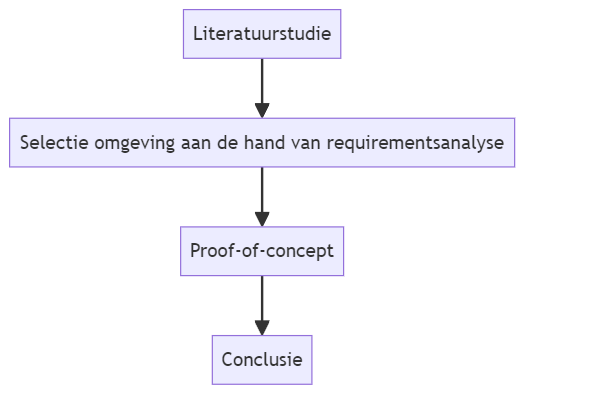
\includegraphics[width=.4\textwidth]{graphics/flowchart.png}
    \caption{\label{fig:flowchart}}Flowchart van methodologie
\end{figure}
%---------- Verwachte resultaten ----------------------------------------------
\section{Verwacht resultaat, conclusie}%
\label{sec:verwachte_resultaten}
Op basis van literatuuronderzoek zal gekozen worden om Bun te vergelijken met Node.js doordat dit framework zich focust op performantie.
De verwachte resultaten zijn metingen van de proof-of-concepts die aantonen dat Bun performanter is dan de Node.js (zie figuur~\ref{fig:uitvoeringstijd} en~\ref{fig:responstijd}). 
Deze metingen werden uitgevoerd met behulp van benchmark tools Hyperfine en Bombardier.
Ook wordt verwacht dat de package manager van Bun een snellere installatietijd heeft dan de Node Package Manager en dat Bun minder complex is dan Node.js (zie figuur~\ref{fig:installatietijd}).
Deze verwachtingen komen mede doordat Bun zich bij de ontwikkeling specifiek heeft gefocust op performantie-optimalisatie.
Ook heeft Bun redelijk wat zaken, zoals een test-runner, al ingebouwd wat het minder complex maakt dan Node.js.
Op basis van deze metingen kan een onderbouwde keuze worden gemaakt tussen het gebruik van Node.js en Bun bij de ontwikkeling
van performante webapplicaties.

Doordat Node.js nog altijd de norm is, zal het zeer veel tijd vragen tegen dat Bun deze effectief kan vervangen.
Het is toch belangrijk dat er nu een keuze kan gemaakt worden tussen javascript runtime-omgevingen bij de ontwikkeling van applicaties.

\begin{figure}
    \centering
    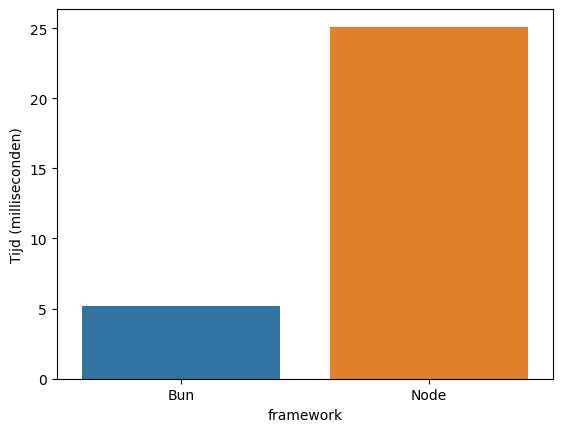
\includegraphics[width=.4\textwidth]{graphics/diagram.png}
    \caption{\label{fig:uitvoeringstijd}}Mock-up waarbij we zien dat Bun een betere uitvoeringstijd heeft dan Node.js bij de uitvoering van een simpel algoritme.
    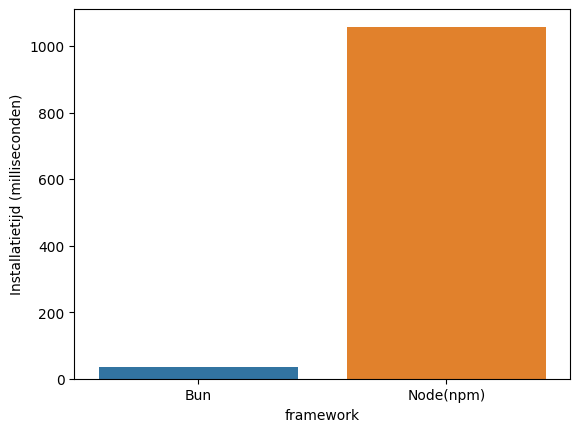
\includegraphics[width=.4\textwidth]{graphics/installatietijd.png}
    \caption{\label{fig:installatietijd}}Mock-up waarbij we zien dat Bun een betere installatietijd heeft dan Node.js bij het installeren van dependencies.
    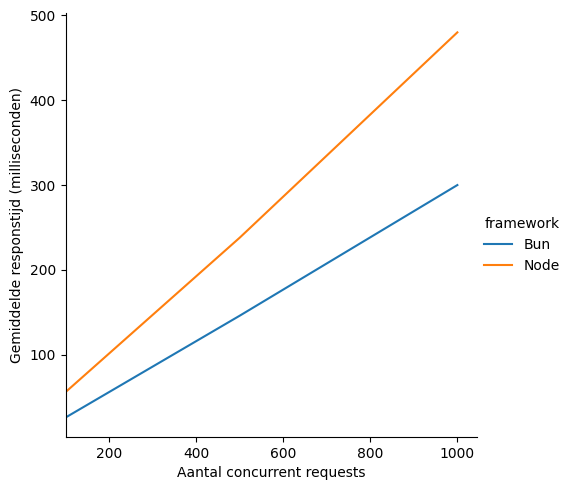
\includegraphics[width=.4\textwidth]{graphics/Responstijd.png}
    \caption{\label{fig:responstijd}}Mock-up waarbij we zien dat Bun een betere responstijd heeft dan Node.js bij het afhandelen van concurrent requests.
\end{figure}
